%%%%%%%%%%%%%%%%%%%%%%%%%%%%%%%%%%%%%%%%%
% Beamer Presentation
% LaTeX Template
% Version 1.0 (10/11/12)
%
% This template has been downloaded from:
% http://www.LaTeXTemplates.com
%
% License:
% CC BY-NC-SA 3.0 (http://creativecommons.org/licenses/by-nc-sa/3.0/)
%
%%%%%%%%%%%%%%%%%%%%%%%%%%%%%%%%%%%%%%%%%

%----------------------------------------------------------------------------------------
%	PACKAGES AND THEMES
%----------------------------------------------------------------------------------------

%\documentclass[c]{beamer}
\documentclass[notes]{beamer}
\setbeamertemplate{note page}[show only notes]
\input{../OR_common.tex}

\usepackage{array}
\newcolumntype{C}{@{}c@{}}
\newcommand{\bottombox}[1]{\makebox[2em][r]{#1}\hspace*{\tabcolsep}\hspace*{2em}}%
\newcommand{\innerbox}[2]{%
    \begin{tabular}[b]{c|c}
       \rule{2em}{0pt}\rule[-2ex]{0pt}{5ex} & \makebox[2em]{#2} \\\cline{2-2}
       \multicolumn{2}{r}{{#1}\hspace*{1.5\tabcolsep}\hspace*{2em}\rule[-2ex]{0pt}{5ex}}
    \end{tabular}}
\renewcommand{\arraystretch}{1.25}

%%%%%%%%%%%%%%%%%%%%%%%%%%%%%%%%%%%%%%%%%%%%%%%%%%%%%%%%%%%%%%%%%%%%%%%%%%%%%
%%%%%%%%%%%%%%%%%%%%%%%%%%%%%%%%%%%%%%%%%%%%%%%%%%%%%%%%%%%%%%%%%%%%%%%%%%%%%
%%%%%%%%%%%%%%%%%%%%%%%%%%%%%%%%%%%%%%%%%%%%%%%%%%%%%%%%%%%%%%%%%%%%%%%%%%%%%

\title[Introduction]{Unit 4. Network Analysis}

\author{Jordi Villà i Freixa}
\institute[FCTE]{
Universitat de Vic - Universitat Central de Catalunya \\
Study Abroad. Operations Research\\
\medskip
\textit{jordi.villa@uvic.cat}
}
\date{9-16/05, 2023}
\logo{
\includegraphics[width=.1\textwidth]{FCTE}}
\begin{document}

\begin{frame}
\titlepage
\end{frame}


\begin{frame}
    \frametitle{Preliminary}
    This course is strongly based on the monography on Operations Research by Carter, Price and Rabadi \cite{carter}, and in material obtained from different sources (quoted when needed through the slides).
\end{frame}

%%%%%%%%%%%%%%%%%%%%%%%%%%%%%%%%%%%%%%%%%%%%%%%%%%%%%%%%%%%%%%%%%%%%%%%%%%%%%
%%%%%%%%%%%%%%%%%%%%%%%%%%%%%%%%%%%%%%%%%%%%%%%%%%%%%%%%%%%%%%%%%%%%%%%%%%%%%
%%%%%%%%%%%%%%%%%%%%%%%%%%%%%%%%%%%%%%%%%%%%%%%%%%%%%%%%%%%%%%%%%%%%%%%%%%%%%
\section{Introduction}
\begin{frame}
\frametitle{Introduction: Learning outcomes}
\begin{itemize}
  \item Getting familiar with the use of network analysis in OR
  \item Understanding network flow in graphs
  \item Understanding minimum cost network flow problems
  \item Applying network connectivity to LP problems
  \item Solving shortest path problems
  \item Understanding and applying dynamic programming
\end{itemize}
\end{frame}

\begin{frame}{Introduction: The concept}
\begin{itemize}
  \item Network analysis provides a framework for the study of a special class of linear programming problems that can be modeled as network programs.
  \item Some of these problems correspond to a physical or geographical network of elements within a system, while others correspond more abstractly to a graphical approach to planning or grouping or arranging the elements of a system.
\end{itemize}
\begin{center}
    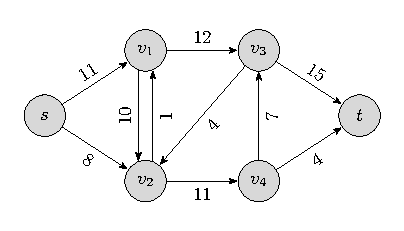
\includegraphics{network.pdf}
\end{center}
\end{frame}

\begin{frame}{Introduction: Examples}
\begin{itemize}
    \item Systems of highways, railroads, shipping lanes, or aviation patterns, where some supply of a commodity is transported or distributed to satisfy a demand;
    \item pipeline systems or utility grids can be viewed as fluid flow or power flow networks;
    \item computer communication networks represent the flow of information;
    \item an economic system may represent the flow of wealth;
    \item routing a vehicle or a commodity between certain specified points in the network; 
    \item assigning jobs to machines, or matching workers with jobs for maximum efficiency; 
    \item project planning and project management, where various activities must be scheduled in order to minimize the duration of a project or to meet specified completion dates, subject to the availability of resources;
    \item and many, many others.
\end{itemize}
\end{frame}

\section{Definitions}

\begin{frame}{Graphs and networks: definitions}
    \begin{center}
    \scalebox{0.5}
    {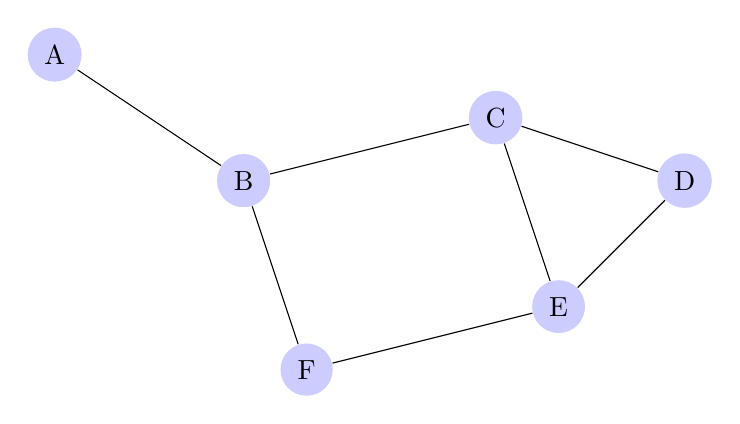
\begin{tikzpicture}
        [scale=.8,auto=left,every node/.style={circle,fill=blue!20}]
        \node (n6) at (1,10) {A};
        \node (n4) at (4,8)  {B};
        \node (n5) at (8,9)  {C};
        \node (n1) at (11,8) {D};
        \node (n2) at (9,6)  {E};
        \node (n3) at (5,5)  {F};    
        \foreach \from/\to in {n6/n4,n4/n5,n5/n1,n1/n2,n2/n5,n2/n3,n3/n4}
          \draw (\from) -- (\to);      
      \end{tikzpicture}
      \begin{tikzpicture}
        [scale=.8,auto=left,every node/.style={circle,fill=blue!20}]
        \node (n6) at (1,10) {A};
        \node (n4) at (4,8)  {B};
        \node (n5) at (8,9)  {C};
        \node (n1) at (11,8) {D};
        \node (n2) at (9,6)  {E};
        \node (n3) at (5,5)  {F};    
        \foreach \from/\to in {n6/n4,n4/n5,n5/n1,n1/n2,n2/n5,n2/n3,n3/n4}
          \draw [-{Stealth[scale=2]}] (\from) -- (\to);      
      \end{tikzpicture}}
    \end{center}
\begin{itemize}
    \item A graph consists of a set of nodes $V$  (vertices, points, or junctions) and a set of connections called arcs $A$ (edges, links, or branches). 
    \item Each connection is associated with a pair of nodes and is usually drawn as a line joining two points. The graph can be defined as directed or undirected. 
    \item The degree of a node is the number of arcs attached to it. An isolated node is of degree zero.
    \item In a directed graph, or digraph, the arc is often designated by the ordered pair $(A, B)$. In digraphs, the direction of the flow matters.
\end{itemize}
\end{frame}

\begin{frame}{Paths}
  \begin{center}
  \begin{tikzpicture}
    [scale=.8,auto=left,every node/.style={circle,fill=blue!20}]
    \node (n6) at (1,10) {A};
    \node (n4) at (4,8)  {B};
    \node (n5) at (8,9)  {C};
    \node (n1) at (11,8) {D};
    \node (n2) at (9,6)  {E};
    \node (n3) at (5,5)  {F};    
    \foreach \from/\to in {n6/n4,n4/n5,n5/n1,n1/n2,n2/n5,n2/n3,n3/n4}
      \draw [-{Stealth[scale=2]}] (\from) -- (\to); 
    \foreach \from/\to in {n5/n1,n1/n2,n2/n5}
      \draw [red, -{Stealth[scale=2]}] (\from) -- (\to);     
  \end{tikzpicture}
\end{center}
\[A,(A,B),B,(B,C),\color{red}{\underbrace{C,(C,D),D,(D,E),E,(E,C),C}_{cyclic}}\]

\end{frame}

\begin{frame}
  \begin{center}
  \begin{tikzpicture}
    [scale=.8,auto=left,every node/.style={circle,fill=blue!20}]
    \node (n6) at (1,10) {A};
    \node (n4) at (4,8)  {B};
    \node (n5) at (8,9)  {C};
    \node (n1) at (11,8) {D};
    \node (n2) at (9,6)  {E};
    \node (n3) at (5,5)  {F};    
    \foreach \from/\to in {n6/n4,n4/n5,n2/n3,n3/n4}
      \draw [-{Stealth[scale=2]}] (\from) -- (\to);      
    \foreach \from/\to in {n5/n1,n1/n2,n5/n2}
      \draw [red,-{Stealth[scale=2]}] (\from) -- (\to);      
  \end{tikzpicture}
\end{center}
\[A,(A,B),B,(B,C),\color{red}{\underbrace{C,(C,D),D,(D,E),E,(C,E),C}_{noncyclic}}\]

\end{frame}

\begin{frame}
  \begin{itemize}
    \item If all the arcs in a path are forward arcs, the path is called {\bf directed chain} or simply {\bf chain}.
    \item {\bf path} and {\bf chain} are synonimous if the graph is undirected.
    \item In the second example above we saw a cyclic path but not a cyclic chain, as it included the backward arc $(C,E)$. 
    \item A {\bf connected graph} has at least one path connecting every pair of nodes.
    \item In a {\bf bipartite graph} the nodes can be partitioned into two subsets $S$ and $T$, such that each node is in exactly one of the subsets, and every arc in the graph connects a node in set $S$ with a node in set $T$.
    \item Such a graph is {\bf complete bipartite} if each node in $S$ is connected to every node in $T$.
  \end{itemize}
\end{frame}

\begin{frame}{Bipartite vs complete bipartite graphs}
  \begin{center}
    \scalebox{0.7}
    {\begin{tikzpicture}[thick,
    every node/.style={draw,circle},
    fsnode/.style={fill=myblue},
    ssnode/.style={fill=mygreen},
    every fit/.style={ellipse,draw,inner sep=-2pt,text width=2cm},
    ->,shorten >= 3pt,shorten <= 3pt
  ]
  
  % the vertices of U
  \begin{scope}[start chain=going below,node distance=7mm]
  \foreach \i in {1,2,...,5}
    \node[fsnode,on chain] (f\i) [label=left: S\i] {};
  \end{scope}
  
  % the vertices of V
  \begin{scope}[xshift=4cm,yshift=-0.5cm,start chain=going below,node distance=7mm]
  \foreach \i in {6,7,...,9}
    \node[ssnode,on chain] (s\i) [label=right: T\i] {};
  \end{scope}
  
  % the set S
  \node [myblue,fit=(f1) (f5),label=above:$S$] {};
  % the set T
  \node [mygreen,fit=(s6) (s9),label=above:$T$] {};
  
  % the edges
  \draw (f1) -- (s6);
  \draw (s6) -- (f2);
  \draw (f2) -- (s7);
  \draw (s7) -- (f3);
  \draw (s8) -- (f3);
  \draw (f3) -- (s9);
  \draw (s9) -- (f5);
  \draw (f5) -- (s6);
  \end{tikzpicture}
  \hspace{3cm}
  \begin{tikzpicture}[thick,
    every node/.style={draw,circle},
    fsnode/.style={fill=myblue},
    ssnode/.style={fill=mygreen},
    every fit/.style={ellipse,draw,inner sep=-2pt,text width=2cm},
    ->,shorten >= 3pt,shorten <= 3pt
  ]
  
  % the vertices of S
  \begin{scope}[start chain=going below,node distance=7mm]
  \foreach \i in {1,2,...,5}
    \node[fsnode,on chain] (f\i) [label=left: S\i] {};
  \end{scope}
  
  % the vertices of T
  \begin{scope}[xshift=4cm,yshift=-0.5cm,start chain=going below,node distance=7mm]
  \foreach \i in {6,7,...,9}
    \node[ssnode,on chain] (s\i) [label=right: T\i] {};
  \end{scope}
  
  % the set S
  \node [myblue,fit=(f1) (f5),label=above:$S$] {};
  % the set T
  \node [mygreen,fit=(s6) (s9),label=above:$T$] {};
  
  % the edges
  \draw (f1) -- (s6);
  \draw (f1) -- (s7);
  \draw (f1) -- (s8);
  \draw (f1) -- (s9);
  \draw (f2) -- (s6);
  \draw (f2) -- (s7);
  \draw (f2) -- (s8);
  \draw (f2) -- (s9);
  \draw (f3) -- (s6);
  \draw (f3) -- (s7);
  \draw (f3) -- (s8);
  \draw (f3) -- (s9);
  \draw (f4) -- (s6);
  \draw (f4) -- (s7);
  \draw (f4) -- (s8);
  \draw (f4) -- (s9);
  \draw (f5) -- (s6);
  \draw (f5) -- (s7);
  \draw (f5) -- (s8);
  \draw (f5) -- (s9);
  \end{tikzpicture}
  }
  \end{center}
\end{frame}

\begin{frame}[allowframebreaks]
  \begin{itemize}
    \item A {\bf tree} is a directed connected graph in which each node has at most on predecessor, and one node (the root node) has none. In an undirected graph, we have a tree if the graph is connected and contains no cycles.
    \begin{center}
    \begin{tikzpicture}[nodes={draw, circle}, -{Stealth[scale=2]}]
    \node{r}
    child { node {a} 
        child { node {c} }
        child { node {d} }
        child { node {e} }
    }
    child [missing]
    child [missing]
    child {node {b} 
        child { node {c} }
        child { node {d} }
        child { node {e} }
    };
  \end{tikzpicture}
\end{center}

    \item A {\bf network} is a directed connected graph that is used to model/represent a system/process. The arcs are typically assigned weights representing cost, value or capacity corresponding to each link.
    \item Nodes in networks can be designated as {\bf sources}, {\bf sinks} or {\bf transshipments}. A {\bf cut set} is any set of arcs which, if removed from the network, would disconnet the sources(s) from the sink(s).
    \item {\bf Flow} can be thought of as the total amount of an entity that originates at the source, makes it through the different nodes and reaches the sink.
  \end{itemize}
\end{frame}

\section{Maximum flow}

\begin{frame}[allowframebreaks]{Maximum flow}
  \begin{block}{Maximum flow in networks}
    Determine the maximum possible flow that can be routed through the various network links, from source ($s$) to sink ($t$), without violating the capacity constraints.

    Important!: the commodity is only generated at the source and consumed at the sink.
  \end{block}

  \begin{center}
    
  
  \begin{tikzpicture}[
    mycircle/.style={
       circle,
       draw=black,
       fill=gray,
       fill opacity = 0.3,
       text opacity=1,
       inner sep=0pt,
       minimum size=20pt,
       font=\small},
    myarrow/.style={-Stealth},
    node distance=0.6cm and 1.2cm
    ]
    \node[mycircle] (c1) {$s$};
    \node[mycircle,below right=of c1] (c2) {$v_2$};
    \node[mycircle,right=of c2] (c3) {$v_4$};
    \node[mycircle,above right=of c1] (c4) {$v_1$};
    \node[mycircle,right=of c4] (c5) {$v_3$};
    \node[mycircle,below right=of c5] (c6) {$t$};

  \foreach \i/\j/\txt/\p in {% start node/end node/text/position
    c1/c2/8/below,
    c1/c4/11/above,
    c2/c3/11/below,
    c3/c6/4/below,
    c4/c5/12/above,
    c5/c6/15/above,
    c5/c2/4/below,
    c3/c5/7/below,
    c2.70/c4.290/1/below}
     \draw [myarrow] (\i) -- node[sloped,font=\small,\p] {\txt} (\j);


   % draw this outside loop to get proper orientation of 10
   \draw [myarrow] (c4.250) -- node[sloped,font=\small,above,rotate=180] {10} (c2.110);
  \end{tikzpicture}
\end{center}
The {\bf maximum flow problem} can be stated as a LP formulation. 
\begin{equation*}
  \begin{aligned}
    \text{maximize } \quad & z = f \\
    \text{subject to }\quad &
    \begin{array}{rcl}
      \sum_{i=2}^n x_{1i}= f&& \\
      \sum_{i=1}^{n-1} x_{in} = f &&\\
      \sum_{i=1}^n x_{ij} = \sum_{k=1}^n x_{jk}, & \text{for } & j=2,3,\ldots,n-1\\
      x_{ij} \leq u_{ij}, & \text{for all } & i,j=1,2,\ldots,n
    \end{array}
  \end{aligned}
\end{equation*}
\note{Constraints (1) and (2) state that all the flow is generated at the source and consumed at the sink. Constraint (1) ensures that a flow of f leaves the source, and because of conservation of flow, that flow stops only at the sink. Constraints (3) are the flow conservation equations for all the intermediate nodes; nothing is generated or consumed at these nodes. Constraints (4) enforce arc capacity restrictions. All flow amounts xij must be non-negative. Actually, constraint (2) is redundant\cite{carter}}
\end{frame}

\begin{frame}{Maximum flow algorithm}
  All network problems here can be solved using the Simplex method, but the network structure can help us solving it more efficiently. In the {\bf Ford-Fulkerson labelling algorithm}:
  \begin{enumerate}
    \item Use a labelling procedure to look for a flow augmenting path. If none can be found, stop; the current flow is optimal;
    \item Increase the current flow as much as possible in the flow augmenting path, until reaching capacity of some arc. Come back to step 1.
  \end{enumerate}
\end{frame}

\begin{frame}
  \begin{Exercise}
    Find the maximum flow in this network using the Ford-Fulkerson labelling algorithm:
  \begin{center}
    
  
    \begin{tikzpicture}[
      mycircle/.style={
         circle,
         draw=black,
         fill=gray,
         fill opacity = 0.3,
         text opacity=1,
         inner sep=0pt,
         minimum size=20pt,
         font=\small},
      myarrow/.style={-Stealth},
      node distance=0.6cm and 1.2cm
      ]
      \node[mycircle] (c1) {$n_1$};
      \node[mycircle,below right=of c1] (c2) {$n_2$};
      \node[mycircle,above right=of c1] (c3) {$n_3$};
      \node[mycircle,above right=of c2] (c4) {$n_4$};
      \node[mycircle,above right=of c4] (c5) {$n_5$};
      \node[mycircle,below right=of c4] (c6) {$n_6$};
      \node[mycircle,above right=of c6] (c7) {$n_7$};
  
    \foreach \i/\j/\txt/\p in {% start node/end node/text/position
      c1/c2/8/below,
      c1/c3/5/above,
      c1/c4/6/above,
      c3/c4/4/above,
      c2/c4/4/below,
      c3/c5/10/above,
      c2/c6/8/below,
      c4/c5/6/above,
      c4/c6/5/below,
      c4/c7/4/above,
      c5/c7/4/above,
      c6/c7/6/below}
       \draw [myarrow] (\i) -- node[sloped,font=\small,\p] {\txt} (\j);
    \end{tikzpicture}
  \end{center}
\end{Exercise}
\note{ Let us assume initially that the flow in all arcs is zero, x ij = 0 and f = 0. In the
first iteration, we label nodes A, B, C, D, and G, and discover the flow augmenting path (A,
D) and (D, G), across which we can increase the flow by 4. So now, x AD = 4, xDG = 4, and f = 4.
In the second iteration, we label nodes A, B, C, then nodes E, D, and F, and finally node G.
A flow augmenting path consists of links (A, B), (B, D), (D, E), and (E, G) and flow on this
path can be increased by 4. Now x AB = 4, xBD = 4, xDE = 4, x EG = 4, and f = 8.
In the third iteration, we see that there remains some unused capacity on link (A, B), so
we can label nodes A, B, and E, but not G. It appears we cannot use the full capacity of link
(A, B). However, we can also label nodes C, D, F, and G, and augment the flow along the
links (A, D), (D, F), and (F, G) by 2, the amount of remaining capacity in (A, D). Now x AD = 6,
xDF = 2, x FG = 2, and f = 10.
In the fourth iteration, we can label nodes A, B, C, D, F, and G. Along the path from A,
C, D, F, to G, we can add a flow of 4, the remaining capacity in (F, G). So x AC = 4, xCF = 4,
x FG = 6, and f = 14.
In the fifth iteration, we can label all nodes except G. Therefore, there is no flow aug-
menting path, and the current flow of 14 is optimal\cite{carter}}
\end{frame}

\begin{frame}
  \begin{itemize}
    \item In any network, there is always a bottleneck that in some sense impedes the flow through the network. 
    \item The total capacity of the bottleneck is an upper bound on the total flow in the network. 
    \item Cut sets are, by definition, essential in order for there to be a flow from source to sink, since removal of the cut set links would render the sink unreachable from the source. 
    \item The capacities on the links in any cut set potentially limit the total flow. 
    \item The minimum cut (i.e., the cut set with minimum total capacity) is in fact the bottleneck that precisely determines the maximum possible flow in the network (Max-Flow Min-Cut Theorem): the capacity of the cut is precisely equal to the current flow and this flow is optimal. In other words, a saturated cut defines the maximum flow.
  \end{itemize}
\end{frame}

\begin{frame}{Multiple sinks and sources}
  We can generate a supersource or  a  supersink node with unlimited capacity and repeat the process of optimization as above:\cite{carter}
  \begin{center}
    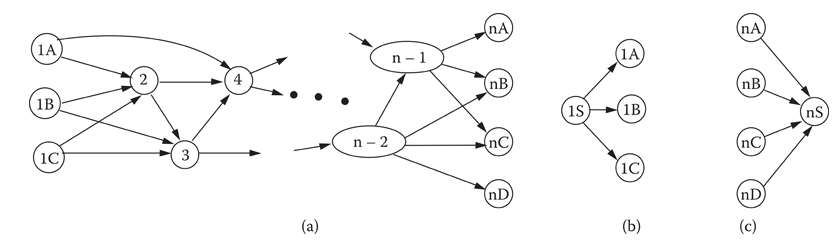
\includegraphics[width=\linewidth]{multiplesinkssources.png}
  \end{center}
\end{frame}

\section{Minimum Cost Network Flow}

\begin{frame}{Transportation problem}
\begin{itemize}
  \item Useful when there are costs associated with the flow, given a link capacity. 
  \item Let us assume that every node is a source (supply) and a sink (demand). Imagine a distributor with several warehouses and a group of costumers. Serving each customer from a given warehouse has an associated cost.
  \item For $m$ supply nodes, each providing $s_i$ suplly,  and $n$ demand nodes, each demanding $d_j$. Assuming that the total demand eaquals the total supply: $\sum_{i=1}^m s_i = \sum_{j=1}^n d_j$ we aim at satisfying the demand using the available supply minimizing cost routes.
\end{itemize}
\end{frame}

\begin{frame}
  \begin{equation*}
    \begin{aligned}
      \text{minimize } \quad & z = \sum_{i=1}^m \sum_{j=1}^n c_{ij}x_{ij} \\
      \text{subject to }\quad &
      \begin{array}{rcl}
        \sum_{j=1}^n x_{ij}= s_i&\text{for }& i=1,\ldots,m \\
        \sum_{i=1}^m x_{ij} = d_j &\text{for }& j=1,\ldots,n \\
        x_{ij} \geq 0 & \text{for all } & i,j
      \end{array}
    \end{aligned}
  \end{equation*}
  \begin{center}
    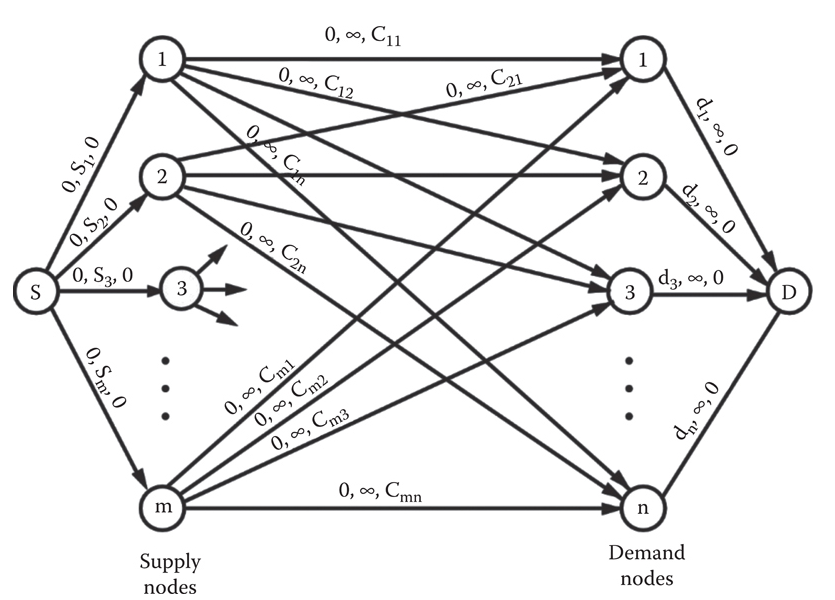
\includegraphics[width=0.55\linewidth]{transportationproblem.png}
  \end{center}
\end{frame}

\begin{frame}
\begin{Exercise}
  Find the minimum cost in this trasportation problem:
  \begin{center}
    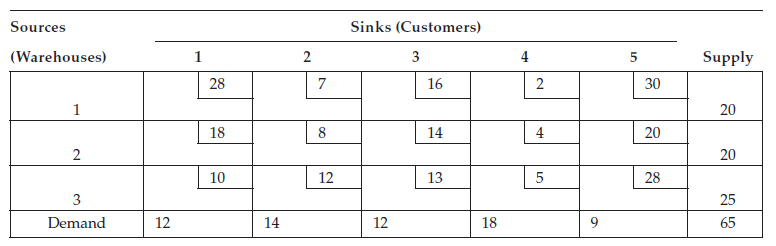
\includegraphics[width=\linewidth]{transportationproblem2.png}
  \end{center}
  NOTE: The Simplex method says that we should first find any basic feasible solution and then look for a simple pivot to improve the solution. repeat until the optimal solution is found.
\end{Exercise}
\end{frame}

\begin{frame}{Optimizing}
\begin{enumerate}
  \item Finding initial solution.
  \begin{itemize}
  \item Northwest corner rule
  \item Minimum cost method
  \item Minimum "row" cost method
  \item Vogel's method (opportunity cost)
  \end{itemize}
  \item Transportation simplex
\end{enumerate}
\end{frame}

\begin{frame}{Transportation simplex}
  Once we have any feasible solution, we aim at finding the optimal one. Consider:
  \begin{center}
    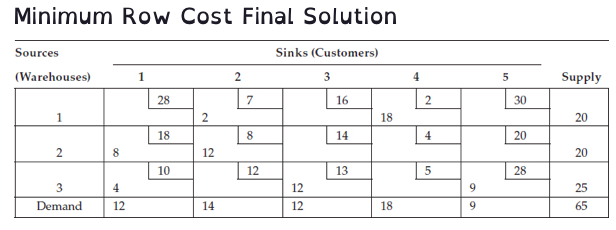
\includegraphics[width=\linewidth]{transportationproblem3.png}
  \end{center}

\end{frame}

\begin{frame}{Transportation simplex}
  We can reduce the total cost by reducing the individual costs in every row $i$ by $u_i$ and in every column $j$ by $v_j$:
  \[c'_{ij}=c_{ij}-u_i-v_j\]
  Check that, now:
  \begin{itemize}
    \item $\sum_i \sum_j x_{ij} c'_{ij}=0$
    \item Check how some costs are now negative in non-basic cells. 
    \item If we increase the number of units in those non-basic cells from 0 to some value, reducing at the same time the number of units in the basic cells, we can reduce the overall cost $\sum_i \sum_j x_{ij} c_{ij}$
  \end{itemize} 

\end{frame}

\begin{frame}{Transportation simplex}
In practice:
\begin{enumerate}
  \item We find first an initial feasible solution as explained above
  \item Calculate the $u_i$ and $v_j$, taking into account that $c_{ij}=u_i+v_j$, for all basic variables (used squares in the table). We start by assigning $u_1=0$.
  \item We calculate the {\em improvement index} by $I_{ij}=c_{ij}-u_i-v_j$ for all non-used squares in the table.
  \item If all $I_{ij}$ are positive, the solution is already optimal and we are done.
  \item If some $I_{ij}<0$, then build a loop with such value in the corner and alternative $\pm$ signs in all vertex. 
  \item Use the above $\pm$ to increase the number of units in the position that had $I_{ij}<0$
  \item We return to step 2.
\end{enumerate}
\end{frame}

% \begin{frame}
%   \resizebox*{\textwidth}{!}{ 
%   \begin{tabular}{c|C|C|C|C|C|r}\hline
%     & 1 & 2 & 3 & 4 & 5 & Supply  \\\hline
% 1   & \innerbox{}{28} & \innerbox{2}{7} & \innerbox{}{16} & \innerbox{18}{2} & \innerbox{}{30} &   20   \\\hline
% 2   & \innerbox{8}{18} & \innerbox{12}{8} & \innerbox{}{14}  & \innerbox{}{4} & \innerbox{}{20}  &   20   \\\hline
% 3   & \innerbox{4}{10} & \innerbox{}{12} & \innerbox{12}{13} & \innerbox{}{5} & \innerbox{9}{28}   &  25   \\\hline
% Demand & \bottombox{12} & \bottombox{14} & \bottombox{12} & \bottombox{18} & \bottombox{9} & 65   \\\hline
% \end{tabular}}
% \end{frame}

\note{dynamic programming: https://www.youtube.com/watch?v=jqyfhFziDjw

https://www.techiedelight.com/word-break-problem/

}
\section{References}
\begin{frame}{References}
    \footnotesize
    \begin{thebibliography}{99}
    \setbeamertemplate{bibliography item}[text]
      \begin{columns}[t]
        \begin{column}{.45\textwidth}
            \bibitem{carter} Michael W. Carter, Camille C. Price, and Ghaith Rabadi. Operations Research, 2nd Edition. CRC Press.
            \bibitem{harel} David Harel, with Yishai Feldman. Algorithmics: the spirit of computing, 3rd Edition. Addison-Wesley.
            \bibitem{rardin} Ronald L. Rardin. Optimization in Operations Research, 2nd Edition. Pearson.
            \bibitem{hefferon} J. Hefferon. \href{http://joshua.smcvt.edu/linearalgebra}{Linear algebra (4th Ed)}.
        \end{column}
        \begin{column}{.45\textwidth}
            \bibitem{riley} K.F. Riley, M.P. Hobson, S.J. Bence. Mathematical Methods for Physics and Engineering (2nd Ed). McGraw Hill.
            \bibitem{nocedal} J. Nocedal, S. J. Wright. Numerical Optimization (2nd Ed). Springer.
            \bibitem{beers} Kenneth J. Beers. Numerical methods for chemical engineering: applications in Matlab. Cambridge University Press.
            \bibitem{barber} D. Barber. Bayesian reasoning and machine learning. Cambridge University Press.
        \end{column}
      \end{columns}
    \end{thebibliography}
\end{frame}
%----------------------------------------------------------------------------------------

\end{document}
